% Vier Gewichte, zerlegt in gemeinsame horizontale Schichten.
% Vektorgrafik: Säulenhöhen sind b_k, Beschriftungen rechts sind Summenbeiträge.
\begin{center}
\begin{minipage}{\linewidth}
\centering
\definecolor{abelLayerOne}{HTML}{DCEAF3}
\definecolor{abelLayerTwo}{HTML}{B8D9D3}
\definecolor{abelLayerThree}{HTML}{E7C995}
\definecolor{abelLayerFour}{HTML}{BDB3D0}
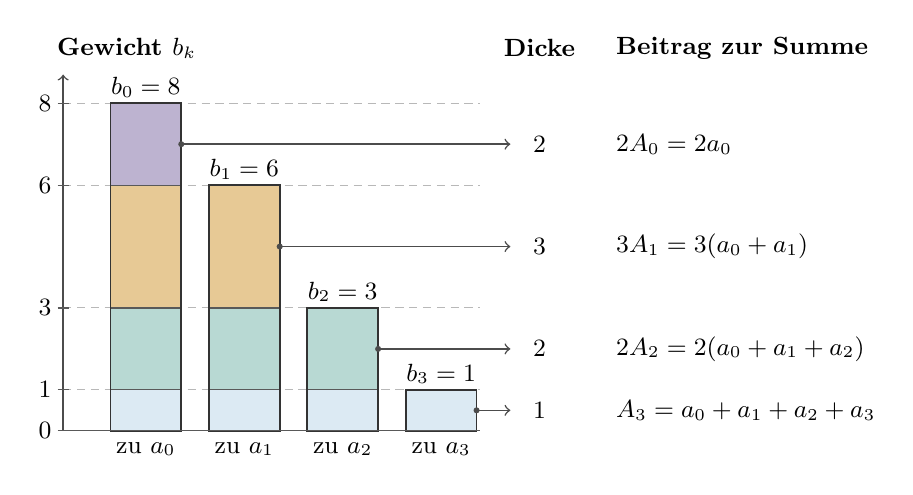
\begin{tikzpicture}[x=1cm,y=.52cm,font=\small,
  layer edge/.style={draw=black!65,line width=.45pt},
  guide/.style={draw=black!28,densely dashed,line width=.35pt},
  contribution/.style={draw=black!70,->,line width=.55pt}]
  % Höhenraster; die ausgefüllten Säulen liegen davor.
  \foreach \height in {1,3,6,8}
    \draw[guide] (0,\height) -- (5.3,\height);
  % Gemeinsame Schichten von unten nach oben.
  \foreach \left in {.6,1.85,3.1,4.35}
    \path[fill=abelLayerOne,layer edge] (\left,0) rectangle +(0.9,1);
  \foreach \left in {.6,1.85,3.1}
    \path[fill=abelLayerTwo,layer edge] (\left,1) rectangle +(0.9,2);
  \foreach \left in {.6,1.85}
    \path[fill=abelLayerThree,layer edge] (\left,3) rectangle +(0.9,3);
  \path[fill=abelLayerFour,layer edge] (.6,6) rectangle +(0.9,2);
  % Konturen und eindeutige Zuordnung zu den Änderungen a_k.
  \foreach \left/\height/\index in {.6/8/0,1.85/6/1,3.1/3/2,4.35/1/3} {
    \draw[black!80,line width=.65pt] (\left,0) rectangle +(0.9,\height);
    \node[above,inner sep=2pt] at ({\left+.45},\height)
      {$b_{\index}=\height$};
    \node[below,inner sep=4pt] at ({\left+.45},0) {zu $a_{\index}$};
  }
  \draw[->,black!70,line width=.55pt] (0,0) -- (0,8.7);
  \draw[black!65,line width=.45pt] (0,0) -- (5.3,0);
  \foreach \height in {0,1,3,6,8} {
    \draw[black!65] (-.07,\height) -- (.07,\height);
    \node[left,inner sep=4pt] at (0,\height) {$\height$};
  }
  \node[anchor=west,font=\small\bfseries] at (-.2,9.35) {Gewicht $b_k$};
  \node[font=\small\bfseries] at (6.05,9.35) {Dicke};
  \node[anchor=west,font=\small\bfseries] at (6.9,9.35) {Beitrag zur Summe};
  % Verbindungen jeweils vom rechten Ende der gesamten Schicht.
  \foreach \right/\middle/\thickness in {5.25/.5/1,4/2/2,2.75/4.5/3,1.5/7/2} {
    \fill[black!70] (\right,\middle) circle[radius=1.1pt];
    \draw[contribution] (\right,\middle) -- (5.68,\middle);
    \node at (6.05,\middle) {$\thickness$};
  }
  \node[anchor=west] at (6.9,.5)
    {$\boldsymbol{A_3}=a_0+a_1+a_2+a_3$};
  \node[anchor=west] at (6.9,2)
    {$\boldsymbol{2A_2}=2(a_0+a_1+a_2)$};
  \node[anchor=west] at (6.9,4.5)
    {$\boldsymbol{3A_1}=3(a_0+a_1)$};
  \node[anchor=west] at (6.9,7)
    {$\boldsymbol{2A_0}=2a_0$};
\end{tikzpicture}
\par\smallskip
{\small\raggedright
Die Säulen zeigen die Gewichte $b_k$. Gleichfarbige Teile bilden
zusammen eine waagerechte Schicht und gewichten ein Anfangsstück
der Änderungen $a_k$. Rechts steht der Beitrag der \emph{ganzen}
Schicht zur gewichteten Summe.\par}
\end{minipage}
\end{center}
